\documentclass[11pt,a4paper]{article}

% Required Packages
\usepackage[utf8]{inputenc}
\usepackage[T1]{fontenc}
\usepackage{lmodern}
\usepackage{amsmath, amssymb}
\usepackage{graphicx}
\usepackage[colorlinks=true,linkcolor=blue!55!black,citecolor=blue!55!black,urlcolor=blue!55!black,pdftitle={Systematic Landscape of Cryptic-Splice Pseudo-Loss-of-Function Variants, ACMG PVS1 Classification Liabilities, and Allele-Specific Antisense Windows Across Five Autosomal-Dominant Dementia Genes},pdfauthor={Manuel Menendez-Gonzalez}]{hyperref}
\usepackage{geometry}
\usepackage{authblk}
\renewcommand\Affilfont{\fontsize{8.5pt}{10.5pt}\selectfont}
\usepackage{cite}
\usepackage{booktabs}
\usepackage{microtype}
\usepackage{setspace}
\usepackage{array}
\usepackage{xcolor}

\geometry{margin=0.92in}
\onehalfspacing
\setlength{\emergencystretch}{2em}

% --- DETERMINISTIC FLOAT PLACEMENT & SECTION-BARRIER ENGINE ---
\renewcommand{\topfraction}{0.95}
\renewcommand{\bottomfraction}{0.95}
\renewcommand{\textfraction}{0.04}
\renewcommand{\floatpagefraction}{0.85}
\setcounter{topnumber}{4}
\setcounter{bottomnumber}{4}
\setcounter{totalnumber}{6}
\setlength{\textfloatsep}{10pt plus 2pt minus 2pt}
\setlength{\floatsep}{8pt plus 2pt minus 2pt}
\setlength{\intextsep}{10pt plus 2pt minus 2pt}
\makeatletter
\newcommand{\FloatBarrier}{%
  \par
  \expandafter\ifx\csname @freelist\endcsname\relax\else
    \ifx\@deferlist\@empty\else
      \clearpage
    \fi
  \fi
}
\let\orig@section\section
\renewcommand{\section}{\FloatBarrier\orig@section}
\makeatother

% --- METADATA ---
\title{Systematic Landscape of Cryptic-Splice Pseudo-Loss-of-Function Variants, ACMG PVS1 Classification Liabilities, and Allele-Specific Antisense Windows Across Five Autosomal-Dominant Dementia Genes}

\author[1,2,3]{Manuel Menendez-Gonzalez\thanks{Corresponding author: \texttt{menendezgmanuel@uniovi.es}}}

\affil[1]{Medicine Department, Oviedo University, Oviedo, Spain}
\affil[2]{Neurology Department, Hospital Universitario Central de Asturias (HUCA), Oviedo, Spain}
\affil[3]{Instituto de Investigaci{\'o}n Sanitaria del Principado de Asturias (ISPA), Oviedo, Spain}

\date{\today}

\begin{document}

\maketitle

\begin{abstract}
Whether dominant dementia mutations act through simple haploinsufficiency or toxic alteration of gene product directly governs clinical variant interpretation and antisense oligonucleotide therapeutics. Following population-genetic and splicing evidence that authentic \textit{PSEN1} null alleles do not cause early-onset Alzheimer's disease (EOAD) whereas the nominal stop-gain \textit{PSEN1} c.325A$>$T (p.K109*) activates a cryptic donor to produce an in-frame deletion (p.K109\_L113del), we constructed a systematic five-gene genomic resource comparing three Alzheimer-linked loci (\textit{PSEN1}, \textit{PSEN2}, \textit{APP}), the tauopathy gene \textit{MAPT}, and the true haploinsufficiency control \textit{GRN}. Across all 1,092 exhaustive GRCh38 MANE Select stop-gain single-nucleotide variants evaluated with AlphaGenome Variant Impact molecular predictions, predicted splicing-disruption attribution (median $\mathrm{fi\_MERGED\_SPLICING}$) was significantly elevated among cryptic-donor and $\leq$2\,bp exon-edge variants compared with interior stop codons ($n=56$, median 0.0898 versus $n=1,036$, median 0.0379; Mann--Whitney $U=42,821.0$, $p=9.35\times 10^{-10}$; Fisher exact odds ratio $5.33$, $p=8.95\times 10^{-6}$ at $\geq 0.25$). Beyond \textit{PSEN1} p.K109* (0.7569, Phred 51.28), the atlas prioritizes additional pseudo-loss-of-function candidates including \textit{PSEN1} p.R308* (1.1523), \textit{PSEN1} p.S102* (c.305C$>$A, 1.1248), \textit{PSEN2} p.W47* (1.0947), \textit{PSEN2} p.K115* (c.343A$>$T, p.K115\_L119del), \textit{APP} p.Y321* (1.1596), and \textit{MAPT} p.G725* (1.2237), contrasted with constrained splicing peaks in \textit{GRN} (maximum 0.5068). Auditing gnomAD v4.1 and 3,368 ClinVar records exposed isoform inflation outside MANE Select in \textit{PSEN2} (5,390 non-MANE alleles) and diagnostic PVS1 classification liabilities across all 11 pathogenic/likely-pathogenic predicted loss-of-function entries in \textit{PSEN1} and \textit{PSEN2}. Cross-species comparison across 29 conserved exons documented sharp decay from exonic (87.7\%) to proximal intronic (45.7\%) identity, explaining why knock-in murine \textit{Psen1} alleles diverge from human cryptic splicing. Cryo-EM contact analysis (PDB 6IYC) and ESM-2 language-model scoring indicated that p.K109\_L113del removes APP-C83 and nicastrin interface contacts within the fifth percentile of 5-residue embedding perturbation ($\mathrm{L2}=0.0769$). Finally, nearest-neighbor thermodynamic scanning identified allele-selective 22-mer steric-blocking antisense windows sparing canonical \texttt{+1/+2\,GU} donors, led by \textit{PSEN1} p.K109* ($\Delta\Delta G^\circ_{37}=+3.63$\,kcal\,mol$^{-1}$, $\Delta T_m=+15.6\,^\circ$C). Together, these computational annotations establish actionable falsifiable hypotheses for clinical genetic curation and experimental validation.
\end{abstract}

\section{Introduction}

Interpreting predicted loss-of-function (pLoF) variants in autosomal-dominant adult-onset dementias presents an enduring mechanistic and diagnostic tension. For genes such as progranulin (\textit{GRN}), nonsense, frameshift, and canonical splice variants cause uniform mRNA degradation via nonsense-mediated decay (NMD) and frontotemporal lobar degeneration through haploinsufficiency~\cite{baker2006}. In contrast, nearly all disease-causing variants in \textit{PSEN1}, \textit{PSEN2}, and \textit{APP} are missense substitutions or in-frame deletions that reshape $\gamma$-secretase substrate proteolysis toward aggregation-prone A$\beta_{42/43}$ species~\cite{zhou2019,arber2019}, while \textit{MAPT} pathogenesis centers on missense alleles and exon 10 stem-loop mutations altering 3R/4R tau isoform stoichiometry~\cite{hutton1998,grover1999}.

Presenilin 1 illustrates the dangers of conflating genetic localization with mechanistic uniformity. Almost two decades ago, Men{\'e}ndez~\cite{menendez2004} documented the broad pathological and clinical heterogeneity of \textit{PSEN1} mutations—spanning spastic paraparesis, cotton-wool plaques, myoclonus, seizures, and extrapyramidal phenotypes—concluding that clinical expression does not track codon position monotonically and likely reflects distinct functional conformations or modifying factors~\cite{menendez2004}. Yet a persistent question remained: could simple allelic dose reduction of \textit{PSEN1} trigger early-onset Alzheimer's disease (EOAD)?

That debate crystallized around a dominantly inherited heterozygous stop-gain variant, \textit{PSEN1} c.325A$>$T (p.K109*), reported in a father--son EOAD duo~\cite{sanjuanruiz2025}. Although homozygous or compound knockouts cause embryonic lethality and true heterozygous LoF variants in \textit{PSEN1}, \textit{PSENEN}, and \textit{NCSTN} cause familial acne inversa (hidradenitis suppurativa) rather than dementia~\cite{wang2010}, overexpression of p.K109* yielded alternative downstream translation products, and aged heterozygous \textit{Psen1}$^{\text{K109*/+}}$ knock-in mice displayed only subtle biochemical changes without plaque pathology~\cite{sanjuanruiz2025}. In a landmark investigation, Farinas et al.~\cite{farinas2026} interrogated the Alzheimer's Disease Sequencing Project, UK Biobank, and BioVU, recovering 45 carriers of high-confidence NMD-triggering \textit{PSEN1} LoF alleles with zero recorded EOAD (including 17 unaffected carriers older than 65 years) and demonstrating that \textit{PSEN1} p.K109* instead creates a \textit{de novo} cryptic splice donor yielding an in-frame 5-amino-acid deletion (p.K109\_L113del)~\cite{farinas2026}.

This discovery carries immediate consequences for clinical genetics and nucleic-acid therapeutics~\cite{menendez2004,farinas2026}. Under American College of Medical Genetics and Genomics / Association for Molecular Pathology (ACMG/AMP) guidelines~\cite{richards2015,aboutayoun2018}, the PVS1 criterion assumes that LoF is an established disease mechanism—an assumption frequently misapplied in diagnostic laboratories when encountering frameshift or splice-site alleles in gain-of-function dementia genes. Moreover, coding sequence changes far inside an exon are rarely evaluated as cryptic splicing activators unless genome-wide splicing predictors are queried systematically~\cite{baralle2005,avsec2026}.

Here, we generalize the cryptic-splice pseudo-LoF paradigm across all five canonical autosomal-dominant dementia loci: \textit{PSEN1}, \textit{PSEN2}, and \textit{APP} (ADAD gain-of-function/processivity loci), \textit{MAPT} (tau isoform splicing/aggregation locus), and \textit{GRN} (true haploinsufficiency control). Combining exhaustive GRCh38 MANE Select stop-gain saturation with live AlphaGenome Variant Impact (AVI) molecular splicing predictions~\cite{avsec2026,alphagenome_atlas2026}, MANE-restricted gnomAD v4.1 constraint auditing~\cite{karczewski2020}, ClinVar PVS1 inspection, human--mouse intronic sequence divergence, cryo-EM $\gamma$-secretase contact geometry (PDB 6IYC)~\cite{zhou2019}, ESM-2 protein language-model perturbation on Apple Silicon GPU~\cite{lin2023}, and nearest-neighbor steric antisense oligonucleotide (ASO) thermodynamics~\cite{santalucia1998}, we build an open, self-contained genomic resource (Research Use Only) to reclassify nominal truncation traps and nominate allele-selective therapeutic windows.

\section{Methods}

\subsection{Five-Gene GRCh38 Transcript Architecture and Exhaustive Stop-Gain Atlas}
Canonical coding sequences and exon boundaries were retrieved from Ensembl GRCh38 for all five targets under their MANE Select transcripts: \textit{PSEN1} (\texttt{ENST00000324501}, chromosome 14, strand $+1$, 467 amino acids), \textit{PSEN2} (\texttt{ENST00000366783}, chromosome 1, strand $+1$, 448 amino acids), \textit{APP} (\texttt{ENST00000346798}, chromosome 21, strand $-1$, 770 amino acids), \textit{MAPT} MANE Select (\texttt{ENST00000262410}, chromosome 17, strand $+1$, 833 amino acids), and \textit{GRN} (\texttt{ENST00000053867}, chromosome 17, strand $+1$, 593 amino acids), alongside the adult brain 2N4R isoform \textit{MAPT\_2N4R} (\texttt{ENST00000344290}, 736 amino acids). Every coding sequence passed start-codon, stop-codon, and peptide-length validation against Ensembl translations.

All single-nucleotide substitutions converting a sense codon to a premature termination codon (\texttt{TAA}, \texttt{TAG}, \texttt{TGA}) were enumerated exhaustively, totaling $n=1,092$ unique variants across the five MANE Select transcripts (\textit{PSEN1} 184, \textit{PSEN2} 151, \textit{APP} 295, \textit{MAPT} 245, \textit{GRN} 217) and 1,307 records including \textit{MAPT\_2N4R} (215). For each stop-gain SNV, our parser annotated: (i) exon length divisibility by 3 (in-frame skippable exons); (ii) penultimate-exon 50-nt NMD escape boundaries; (iii) proximity ($\leq 2$\,bp) to canonical exon boundaries; and (iv) \textit{de novo} \texttt{GT} cryptic donors or \texttt{AG} cryptic acceptors restoring an in-frame junction against position-weight matrix (PWM) motif strengths computed across the native donor/acceptor background.

\subsection{AlphaGenome Variant Impact Molecular Splicing Atlas}
Variant-level splicing predictions were retrieved programmatically from the public AlphaGenome Atlas resource~\cite{avsec2026,alphagenome_atlas2026} across 62 exon and splice-junction genomic intervals (collecting 29,736 scored SNVs overall). Every member of the 1,092 MANE Select stop-gain panel (100\% coverage) and \textit{MAPT\_2N4R} plus canonical splice-site controls was matched to its AlphaGenome splicing attribution metric (\texttt{fi\_MERGED\_SPLICING}) and Phred-scaled variant impact score. For every hit meeting $\mathrm{fi\_MERGED\_SPLICING} \geq 0.25$ ($n=74$ unique SNVs across all isoforms), individual modality tracks and top tissue/cell-type attributions were extracted. Because AlphaGenome outputs are computational molecular phenotypes intended strictly for research use, all splicing attributions were treated as \textit{in silico} hypotheses rather than clinical classifications. Statistical enrichment between cryptic-donor / $\leq 2$\,bp edge candidates ($n=56$) and interior stop codons ($n=1,036$) was evaluated by two-sided Mann--Whitney $U$ and Fisher exact tests ($\mathrm{fi\_MERGED\_SPLICING} \geq 0.25$ cutoff). An orthogonal 108-SNV saturation scan was extracted across the 36-nt boundary window spanning \textit{PSEN1} Exon 4 through Intron 4 ($-27$\,nt to $+9$\,nt relative to \texttt{chr14:73171047}).

\subsection{gnomAD v4.1 MANE Restriction, ClinVar Audit, and PVS1 Adjudication}
Population constraint metrics (\texttt{pLI}, \texttt{oe\_lof\_upper}/LOEUF, \texttt{oe\_lof}, \texttt{oe\_mis}) and all coding/splice variant calls for the five loci were queried from gnomAD v4.1~\cite{karczewski2020}. Because gene-wide gnomAD dumps include non-coding and minority transcript isoforms, we applied a strict coordinate filter restricting pLoF alleles (\texttt{stop\_gained}, \texttt{frameshift\_variant}, \texttt{splice\_donor\_variant}, \texttt{splice\_acceptor\_variant}, \texttt{start\_lost}) to coding exons $\pm 5$\,bp of the MANE Select transcript. In parallel, all 3,368 ClinVar variants across the five genes (\textit{PSEN1} 659, \textit{PSEN2} 421, \textit{APP} 730, \textit{MAPT} 691, \textit{GRN} 867) were harvested and partitioned into missense, in-frame indel, and pLoF Pathogenic/Likely Pathogenic (P/LP) assertions. Every P/LP pLoF entry in \textit{PSEN1} ($n=8$) and \textit{PSEN2} ($n=3$) was inspected at submitter, assertion-criteria, and citation levels against ClinGen Sequence Variant Interpretation PVS1 rules~\cite{richards2015,aboutayoun2018}.

\subsection{Human--Mouse Exonic vs.\ Intronic Junction Divergence}
To quantify evolutionary conservation across splice-regulatory contexts, human exonic 60-bp termini and adjacent 60-bp proximal intronic sequences for exons harboring top AlphaGenome stop-gain hits were aligned against mouse GRCm39 orthologs via Ensembl comparative exons. Analyses focused on length-matched conserved coding exons ($n=29$, defined conservatively as $|\text{len}_{\text{human}} - \text{len}_{\text{mouse}}| \leq 15$\,bp and 60-bp exonic identity $\geq 0.70$).

\subsection{Cryo-EM Geometry, ESM-2 Protein Language Modeling, and Steric ASO Design}
Hydrophilic loop 1 (HL1, residues 100--139) of \textit{PSEN1} was inspected in the substrate-bound cryo-EM structure of human $\gamma$-secretase complexed with APP-C83 (PDB ID \texttt{6IYC}; chain A nicastrin, B \textit{PSEN1}[Q112C], C APH-1A, D PEN-2, E APP-C83[V8C])~\cite{zhou2019}. Minimum heavy-atom distances from each HL1 residue to APP-C83, nicastrin, PEN-2, and the catalytic aspartates (D257, D385), as well as the C$\alpha$ bridge distance across R108--I114, were computed in Python. Unmodeled residues (including S290 vs.\ residues 308--319 of Exon 9) were documented explicitly.

Full-length wild-type and in-frame deletion mutant sequences (six cryptic-donor deletions plus \textit{PSEN1} $\Delta\text{Exon 9}$, contrasted against 20 random 5-amino-acid internal deletions along \textit{PSEN1}) were embedded using \texttt{facebook/esm2\_t12\_35M\_UR50D}~\cite{lin2023} on an Apple M4 Max GPU (PyTorch 2.14.1, \texttt{mps} backend). Global sequence L2 embedding shift, mean pseudo-log-likelihood change ($\Delta\mathrm{PLL}$), and flanking 10-residue local PLL were computed.

Allele-selective steric-blocking 22-mer RNA ASO windows tiling 61-nt pre-mRNA targets around 32 high-priority stop-gain splice hotspots were evaluated using unified nearest-neighbor thermodynamics ($\Delta G^\circ_{37}$ and predicted $T_m$ for mutant versus wild-type RNA duplexes)~\cite{santalucia1998}, hairpin self-complementarity bounds, and an explicit filter excluding oligos overlapping canonical \texttt{+1/+2\,GU} splice donors to avoid off-target wild-type splice inhibition. All classified variants and ASO candidates were formalized into a schema-validated GeneForge Language (\texttt{.gfl}) specification passing parser and static validation with zero errors.

\section{Results}

\subsection{Constraint Divergence, MANE Isoform Inflation, and ClinVar Asymmetry Across Five Loci}
Systematic integration of gnomAD v4.1 and ClinVar across the five loci revealed a sharp dichotomy between disease mechanism and summary constraint metrics (\textbf{Table~\ref{tab:five_gene_overview}}, \textbf{Figure~\ref{fig:fig1}}). Both \textit{PSEN1} ($\mathrm{pLI}=0.9995$, $\mathrm{LOEUF}=0.432$) and \textit{APP} ($\mathrm{pLI}=1.0000$, $\mathrm{LOEUF}=0.413$) exhibit strong germline pLoF depletion despite causing ADAD through altered proteolysis or dosage rather than coding null haploinsufficiency; conversely, the true haploinsufficiency locus \textit{GRN} presents intermediate constraint ($\mathrm{pLI}=0.0149$, $\mathrm{LOEUF}=0.610$) yet harbors 124 P/LP pLoF variants out of 132 total P/LP entries in ClinVar (93.9\% pLoF enrichment; missense P/LP = 8).

\begin{table}[!htb]
\centering
\caption{Five-gene GRCh38 MANE Select architecture, gnomAD v4.1 constraint (total versus MANE-restricted pLoFs), ClinVar pathogenicity breakdown, and AlphaGenome stop-gain splicing summary.}
\label{tab:five_gene_overview}
\footnotesize
\setlength{\tabcolsep}{3pt}
\resizebox{\textwidth}{!}{%
\begin{tabular}{@{}lccccccccc@{}}
\toprule
Gene & \shortstack{MANE\\(aa)} & \shortstack{Stop\\SNVs} & \shortstack{pLI /\\LOEUF} & \shortstack{gnomAD\\pLoF (AC)} & \shortstack{MANE\\pLoF (AC)} & \shortstack{CV\\Total} & \shortstack{CV Mis\\P/LP} & \shortstack{CV pLoF\\P/LP} & \shortstack{AG $\geq 0.25$\\$n$ (\%)} \\
\midrule
\textit{PSEN1} & 467 & 184 & 0.9995 / 0.432 & 83 (206)   & 74 (198)  & 659 & 139 & 8   & 9 (4.89\%) \\
\textit{PSEN2} & 448 & 151 & 0.0000 / 0.876 & 149 (6,226)& 96 (836)  & 421 & 8   & 3   & 13 (8.61\%) \\
\textit{APP}   & 770 & 295 & 1.0000 / 0.413 & 81 (231)   & 73 (216)  & 730 & 28  & 0   & 18 (6.10\%) \\
\textit{MAPT}  & 833 & 245 & 0.0002 / 0.666 & 224 (923)  & 167 (746) & 691 & 25  & 0   & 25 (10.20\%) \\
\textit{GRN}   & 593 & 217 & 0.0149 / 0.610 & 154 (371)  & 142 (341) & 867 & 8   & 124 & 10 (4.61\%) \\
\bottomrule
\end{tabular}%
}
\end{table}

Crucially, restricting gnomAD v4.1 records strictly to MANE Select coding exons ($\pm 5$\,bp) uncovered severe transcript-isoform inflation in \textit{PSEN2}: of 6,226 raw pLoF alleles reported gene-wide (149 variant records), 5,390 alleles (86.6\%, across 53 records) mapped outside the MANE Select \texttt{ENST00000366783} coding scaffold. Even after MANE filtering, \textit{PSEN2} retained 96 coding/canonical-splice pLoF sites totaling 836 alleles in the general population (median-unconstrained $\mathrm{pLI}=0.0000$, $\mathrm{LOEUF}=0.876$), led by the start-lost allele \texttt{1-226888112-A-G} ($\mathrm{AC}=617$) and an Exon 5 frameshift deletion (\texttt{1-226883897-TAC-T}, $\mathrm{AC}=13$) lying merely 6\,bp from the familial Alzheimer variant \textit{PSEN2} p.K115fs. In \textit{APP} and \textit{MAPT}, zero P/LP pLoF assertions appear among 1,421 combined ClinVar variants (though \textit{MAPT} holds one pathogenic in-frame deletion, \texttt{p.Asn688del}).

\begin{figure}[!htb]
  \centering
  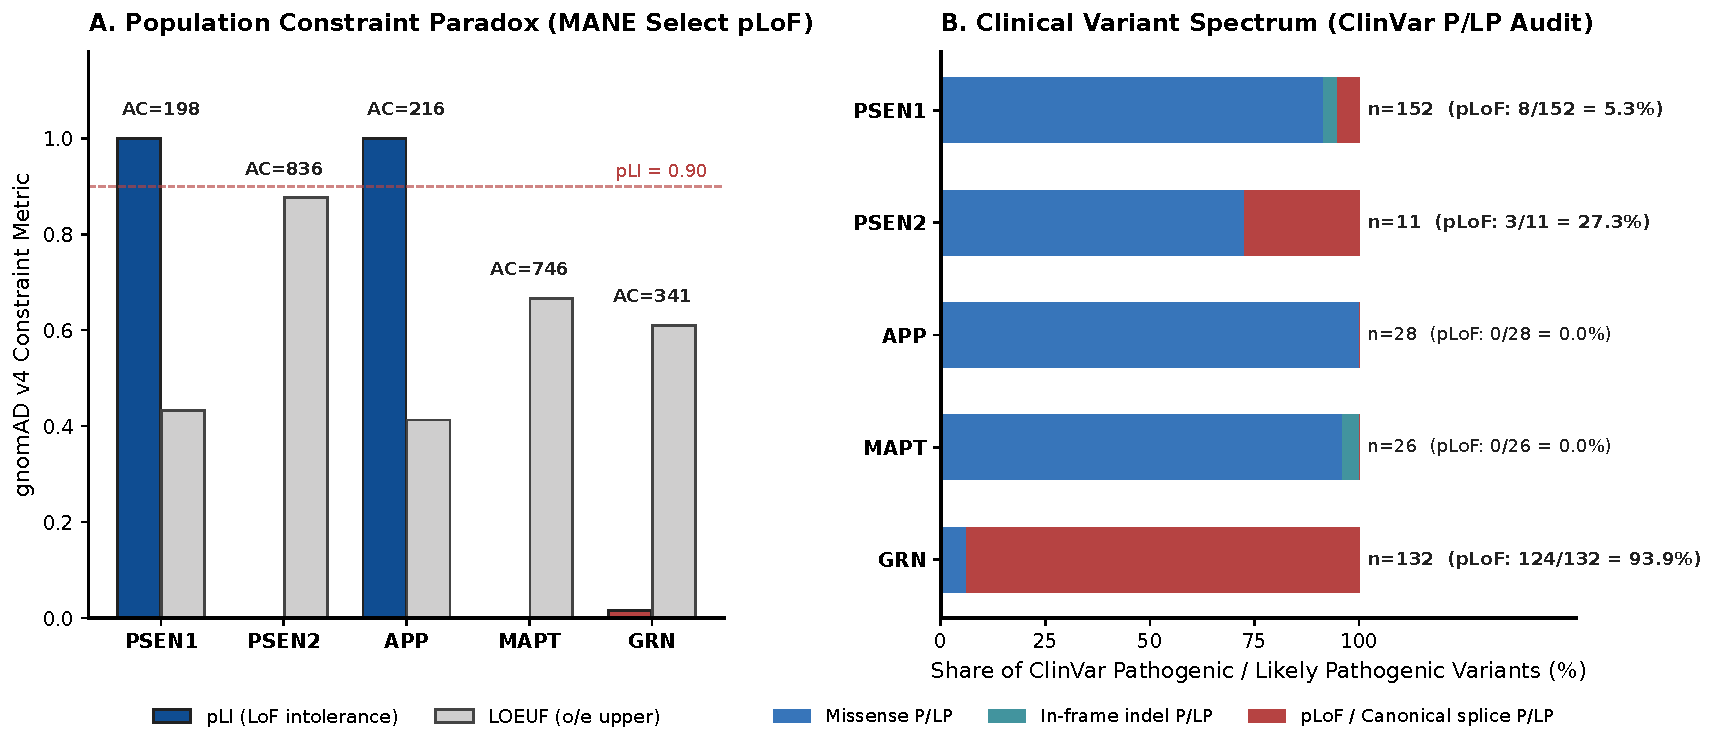
\includegraphics[width=0.96\textwidth,height=0.45\textheight,keepaspectratio]{figures/fig1_five_gene_constraint_clinvar.pdf}
  \caption{Population intolerance and ClinVar clinical variant spectrum across five dementia genes. \textbf{(A)} gnomAD v4.1 \texttt{pLI} and \texttt{LOEUF} constraint metrics alongside MANE Select coding/canonical-splice pLoF allele counts (\texttt{AC}); for \textit{PSEN2}, MANE restriction excludes 5,390 of 6,226 raw gene-wide pLoF alleles located outside the canonical scaffold. \textbf{(B)} ClinVar Pathogenic / Likely Pathogenic variant composition partitioned into missense, in-frame indel, and nominal pLoF / canonical splice classes (total P/LP counts and pLoF percentages shown at right).}
  \label{fig:fig1}
\end{figure}

Structural taxonomy of the 1,092 MANE Select stop-gain SNVs further demonstrated that large fractions reside inside exons whose lengths are exact multiples of 3 or past the 50-nt penultimate NMD escape threshold: 86/184 (46.7\%) in \textit{PSEN1} (skippable exons 8 [99\,bp], 9 [87\,bp], 10 [174\,bp]; NMD escape $\geq\mathrm{aa}\,398$), 63/151 (41.7\%) in \textit{PSEN2} (exons 9, 10, 11; NMD escape $\geq\mathrm{aa}\,379$), 170/295 (57.6\%) in \textit{APP} (nine skippable exons; NMD escape $\geq\mathrm{aa}\,719$), 177/245 (72.2\%) in \textit{MAPT} (five skippable exons; NMD escape $\geq\mathrm{aa}\,744$), and 134/217 (61.8\%) in \textit{GRN} (four skippable exons; NMD escape $\geq\mathrm{aa}\,530$). Sequence motif scanning across the four non-\textit{GRN} dementia loci also flagged candidate \textit{de novo} in-frame cryptic donors directly induced by stop codons: \textit{PSEN1} p.K109* (\texttt{c.325A>T}, Exon 4, deleting 5 aa via \texttt{CCG|GTAGGA}, PWM 11.7 vs.\ native 10.0), \textit{PSEN1} p.Q112* (\texttt{c.334C>T}, Exon 4, 2 aa \texttt{TGG|GTAGCT}), \textit{PSEN1} p.Y181* (\texttt{c.543C>G}, Exon 6, 2 aa), \textit{PSEN2} p.K115* (\texttt{c.343A>T}, Exon 5, deleting 5 aa \texttt{KNGQL} via \texttt{AGA|GTAGAA}, PWM 8.1 vs.\ native 11.2), and \textit{APP} p.E202* and p.E203* (Exon 5, 20-aa and 19-aa deletions).

\subsection{Pan-Gene AlphaGenome Splicing Attribution Atlas Across 1,092 Stop-Gain SNVs}
Evaluation of all 1,092 MANE Select stop-gain SNVs via AlphaGenome Variant Impact (\texttt{fi\_MERGED\_SPLICING}) revealed strong statistical enrichment of splicing disruption among cryptic-donor and $\leq 2$\,bp exon-edge nonsense mutations relative to interior stop codons (\textbf{Figure~\ref{fig:fig2}}). Across the full five-gene corpus, candidate cryptic-donor or boundary variants ($n=56$, median 0.0898) scored more than twofold higher than interior stop codons ($n=1,036$, median 0.0379; Mann--Whitney $U=42,821.0$, $p=9.35\times 10^{-10}$) and were 5.33-fold enriched above $\mathrm{fi\_MERGED\_SPLICING} \geq 0.25$ (14/56 vs.\ 61/1,036; Fisher exact $p=8.95\times 10^{-6}$).

\begin{figure}[!htb]
  \centering
  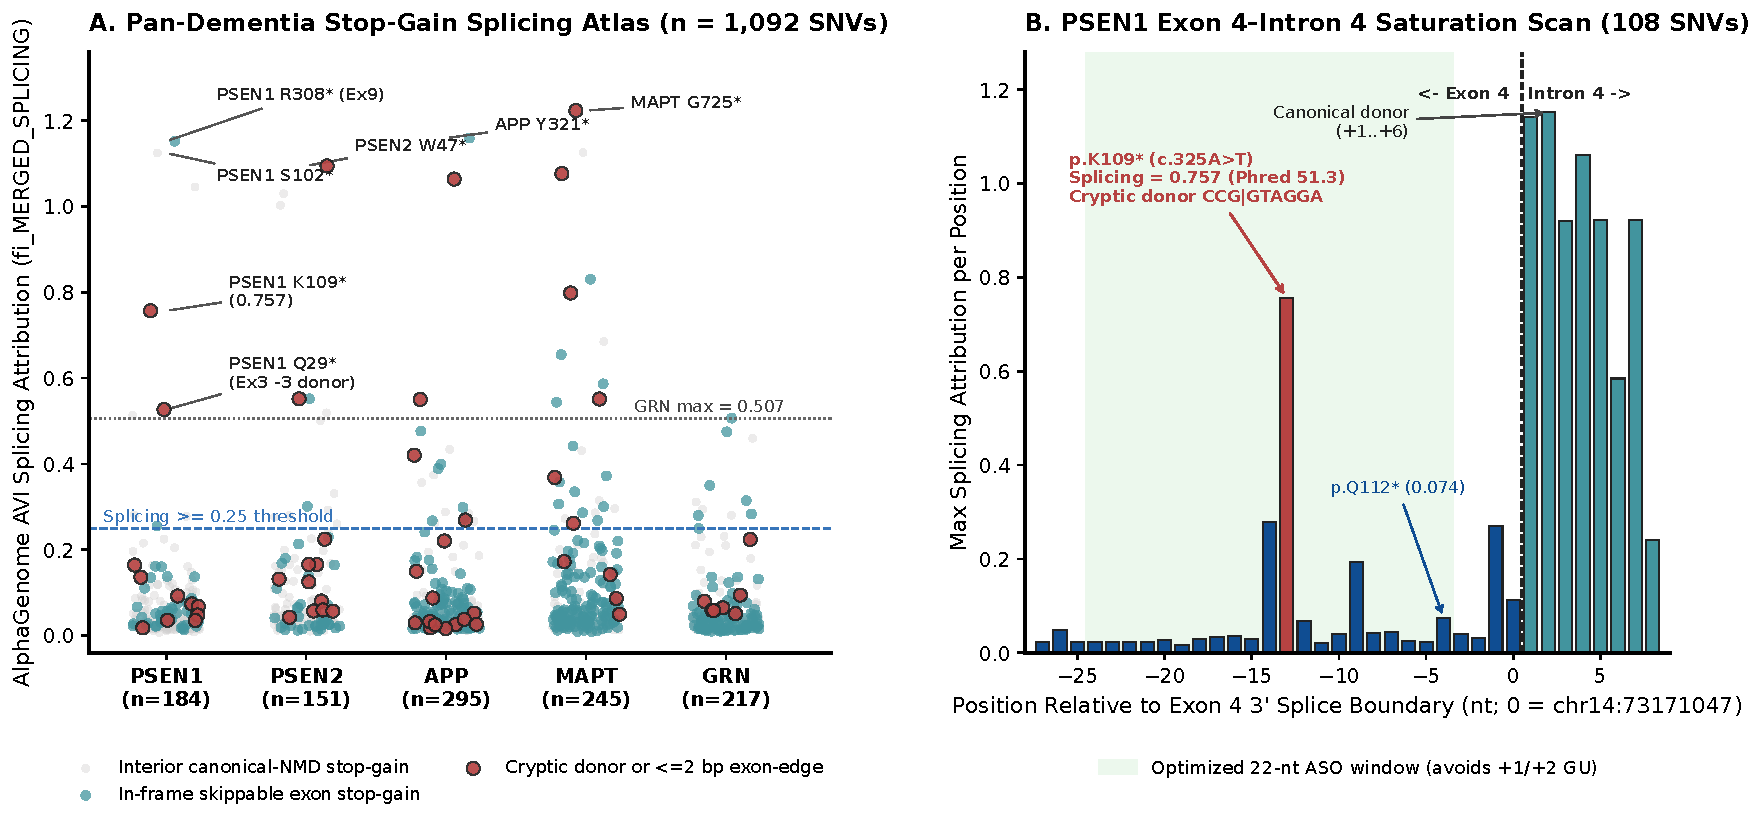
\includegraphics[width=0.96\textwidth,height=0.45\textheight,keepaspectratio]{figures/fig2_alphagenome_stopgain_splicing_atlas.pdf}
  \caption{Pan-dementia AlphaGenome stop-gain splicing attribution atlas and saturation dissection of the \textit{PSEN1} Exon 4--Intron 4 boundary. \textbf{(A)} Distribution of \texttt{fi\_MERGED\_SPLICING} scores across all 1,092 MANE Select stop-gain SNVs, highlighting high-impact pseudo-LoF candidates in \textit{PSEN1} (p.R308*, p.S102*, p.K109*, p.Q29*), \textit{PSEN2} (p.W47*), \textit{APP} (p.Y321*), and \textit{MAPT} (p.G725*) against the ceiling of \textit{GRN} (max 0.507). \textbf{(B)} Per-position maximum AlphaGenome splicing attribution across all 108 possible SNVs spanning \textit{PSEN1} Exon 4 ($-27$\,nt to $-1$\,nt) and Intron 4 ($+1$\,nt to $+9$\,nt), demonstrating that \textit{PSEN1} p.K109* (0.7569, Phred 51.28) produces the strongest exonic signal while the proximal cryptic donor p.Q112* scores near baseline (0.0737). Shaded green window indicates the optimized 22-mer ASO steric window avoiding canonical \texttt{+1/+2\,GU}.}
  \label{fig:fig2}
\end{figure}

Gene-level summary statistics revealed stark divergence between the gain-of-function/isoform dementia genes and the true LoF control \textit{GRN} (\textbf{Table~\ref{tab:five_gene_overview}}). Extreme splicing peaks (splicing attribution $\geq 0.50$) were frequent in \textit{PSEN1} (6/184, max 1.1523), \textit{PSEN2} (7/151, max 1.0947), \textit{APP} (3/295, max 1.1596), and \textit{MAPT} (10/245, max 1.2237, driven by Ammon's horn / brain-enriched splice tracks for p.G725* near Exon 11 and p.K24*), whereas \textit{GRN} exhibited only a single borderline hit above 0.50 (p.C410*, max 0.5068; overall median 0.0359, IQR 0.0371, mean Phred 32.66).

Within \textit{PSEN1}, the 108-SNV saturation scan of the Exon 4--Intron 4 junction (\textbf{Figure~\ref{fig:fig2}B}) established that c.325A$>$T (p.K109*) ranks first overall among all exonic positions in both Phred impact (51.28) and splicing attribution (0.7569), exceeded solely by canonical Intron 4 \texttt{+1} to \texttt{+7} donor positions (0.836--1.151). By contrast, a sequence-matched downstream \textit{de novo} \texttt{GT} motif three codons closer to the junction, \textit{PSEN1} c.334C$>$T (p.Q112*), received minimal attribution (0.0737, Phred 40.75), as did \textit{PSEN2} p.K115* (0.0570) and \textit{APP} p.E202*/E203* (0.0254/0.0262)—underscoring the necessity of full sequence-context modeling over local PWM rules alone. Crucially, AlphaGenome surfaced additional internal or exon-edge stop-gain hotspots across \textit{PSEN1} that had not previously been recognized as pseudo-LoF candidates: c.922A$>$T (p.R308*, Exon 9 87-bp in-frame module, splicing 1.1523, Phred 59.46), c.305C$>$A (p.S102*, Exon 4 internal exonic splicing enhancer/motif, 1.1248, Phred 61.83; c.305C$>$G scores 0.5132), and c.85C$>$T (p.Q29*, Exon 3 position $-3$ converting \texttt{CAG|GTACAG} to \texttt{TAG|GTACAG}, 0.5266, Phred 51.01).

\subsection{Dissection of ACMG PVS1 Liabilities in ClinVar and Human--Mouse Intronic Divergence}
Inspection of all 11 P/LP pLoF records currently hosted in ClinVar for \textit{PSEN1} ($n=8$) and \textit{PSEN2} ($n=3$) exposed three recurring PVS1 classification liabilities (\textbf{Table~\ref{tab:clinvar_traps}}). Five \textit{PSEN1} entries correspond directly to the classical in-frame 87-bp Exon 9 skipping ($\Delta\text{E9}$) mechanism (\texttt{c.869-2A>G}, \texttt{c.869-1G>A}, \texttt{c.869-2A>T}, \texttt{c.869-1G>T}, and genomic deletion \texttt{c.869-1624\_956-2452del})~\cite{pereztur1995}; one represents the well-characterized Intron 4 deletion \texttt{c.338+1del} activating cryptic splicing to produce in-frame p.T113\_I114insT~\cite{dejonghe1999,arber2019}; and one (\texttt{c.725del}, p.Pro242fs) is asserted solely for familial Acne Inversa 3 rather than ADAD~\cite{wang2010}. Notably, the sole remaining nonsense submission in \textit{PSEN1}—ClinVar ID \texttt{1027511} (\texttt{c.300dup}, p.Lys101Ter, Pathogenic, single submitter 2021)—carries zero peer-reviewed citations and sits four nucleotides upstream of the \textit{PSEN1} c.305C$>$A (p.S102*) splicing hotspot, leaving unresolved whether it represents a rare unverified pseudo-LoF splice trap or an erroneous PVS1 assignment.

\begin{table}[!htb]
\centering
\caption{Evidence-level audit of all 11 ClinVar Pathogenic / Likely Pathogenic predicted loss-of-function entries in \textit{PSEN1} and \textit{PSEN2}.}
\label{tab:clinvar_traps}
\footnotesize
\setlength{\tabcolsep}{3pt}
\resizebox{\textwidth}{!}{%
\begin{tabular}{@{}lllll>{\raggedright\arraybackslash}p{4.8cm}@{}}
\toprule
Gene & ID & Variant (MANE) & Submitter (Date) & Cites & Mechanistic Audit / PVS1 Verdict \\
\midrule
\textit{PSEN1} & 2925523 & \texttt{c.869-2A>G} & Labcorp/Invitae (2022) & 4 & In-frame $\Delta$E9 (87 bp); pseudo-LoF GoF~\cite{pereztur1995} \\
\textit{PSEN1} & 599622  & \texttt{c.869-1G>A} & Multiple (2023) & 11 & In-frame $\Delta$E9 (87 bp); pseudo-LoF GoF \\
\textit{PSEN1} & 579680  & \texttt{c.869-2A>T} & Labcorp/Invitae (2018) & 3 & In-frame $\Delta$E9 (87 bp); pseudo-LoF GoF \\
\textit{PSEN1} & 98092   & \texttt{c.869-1G>T} & OMIM/VIB (2001) & 6 & In-frame $\Delta$E9 (87 bp); pseudo-LoF GoF~\cite{pereztur1995} \\
\textit{PSEN1} & 38296   & \texttt{c.869-1624\_956-2452del} & GeneReviews (2010) & 2 & Genomic $\Delta$E9 deletion; pseudo-LoF GoF \\
\textit{PSEN1} & 98013   & \texttt{c.338+1del} & Athena / OMIM (2021) & 11 & Cryptic donor $\rightarrow$ p.T113\_I114insT~\cite{dejonghe1999,arber2019} \\
\textit{PSEN1} & 29606   & \texttt{c.725del} (p.P242fs) & OMIM (2010) & 1 & Familial Acne Inversa 3, NOT EOAD~\cite{wang2010} \\
\textit{PSEN1} & 1027511 & \texttt{c.300dup} (p.K101*) & IRCCS Stella Maris (2021) & 0 & Uncited single submission; 4 nt from S102* \\
\midrule
\textit{PSEN2} & 3720283 & \texttt{c.342\_343del} (p.K115fs) & Labcorp/Invitae (2024) & 4 & pLI=0; adj.\ fs AC=13; PS2V model~\cite{jayadev2010,hin2020} \\
\textit{PSEN2} & 4726843 & \texttt{c.356+2T>C} & Labcorp/Invitae (2025) & 4 & Intron 5 donor; PVS1 unsupported~\cite{farinas2026} \\
\textit{PSEN2} & 465218  & \texttt{c.886+2\_886+4del} & Labcorp/Invitae (2017) & 4 & 99-bp skippable Ex9; requires PVS1 downgrade \\
\bottomrule
\end{tabular}%
}
\end{table}

Equally concerning, all three P/LP pLoF records in \textit{PSEN2} (ClinVar ID~3720283, \texttt{c.342\_343del} p.Lys115fs, Pathogenic 2024; ID~4726843, \texttt{c.356+2T>C}, Likely Pathogenic 2025; ID~465218, \texttt{c.886+2\_886+4del}, Likely Pathogenic 2017) originate from single-submitter pipelines invoking Sherloc rules~\cite{richards2015,aboutayoun2018}. Yet \textit{PSEN2} has $\mathrm{pLI}=0.0000$, carries 836 MANE coding pLoF alleles (including a common benign frameshift 6\,bp from p.K115fs), and variant \texttt{c.886+2\_886+4del} disrupts the donor of Exon 9—an exact 99-bp in-frame skippable exon whose deletion preserves reading frame (\textbf{Figure~\ref{fig:fig3}A}). Thus, diagnostic assertions resting upon canonical LoF premises in \textit{PSEN1} or \textit{PSEN2} require mandatory re-evaluation.

\begin{figure}[!htb]
  \centering
  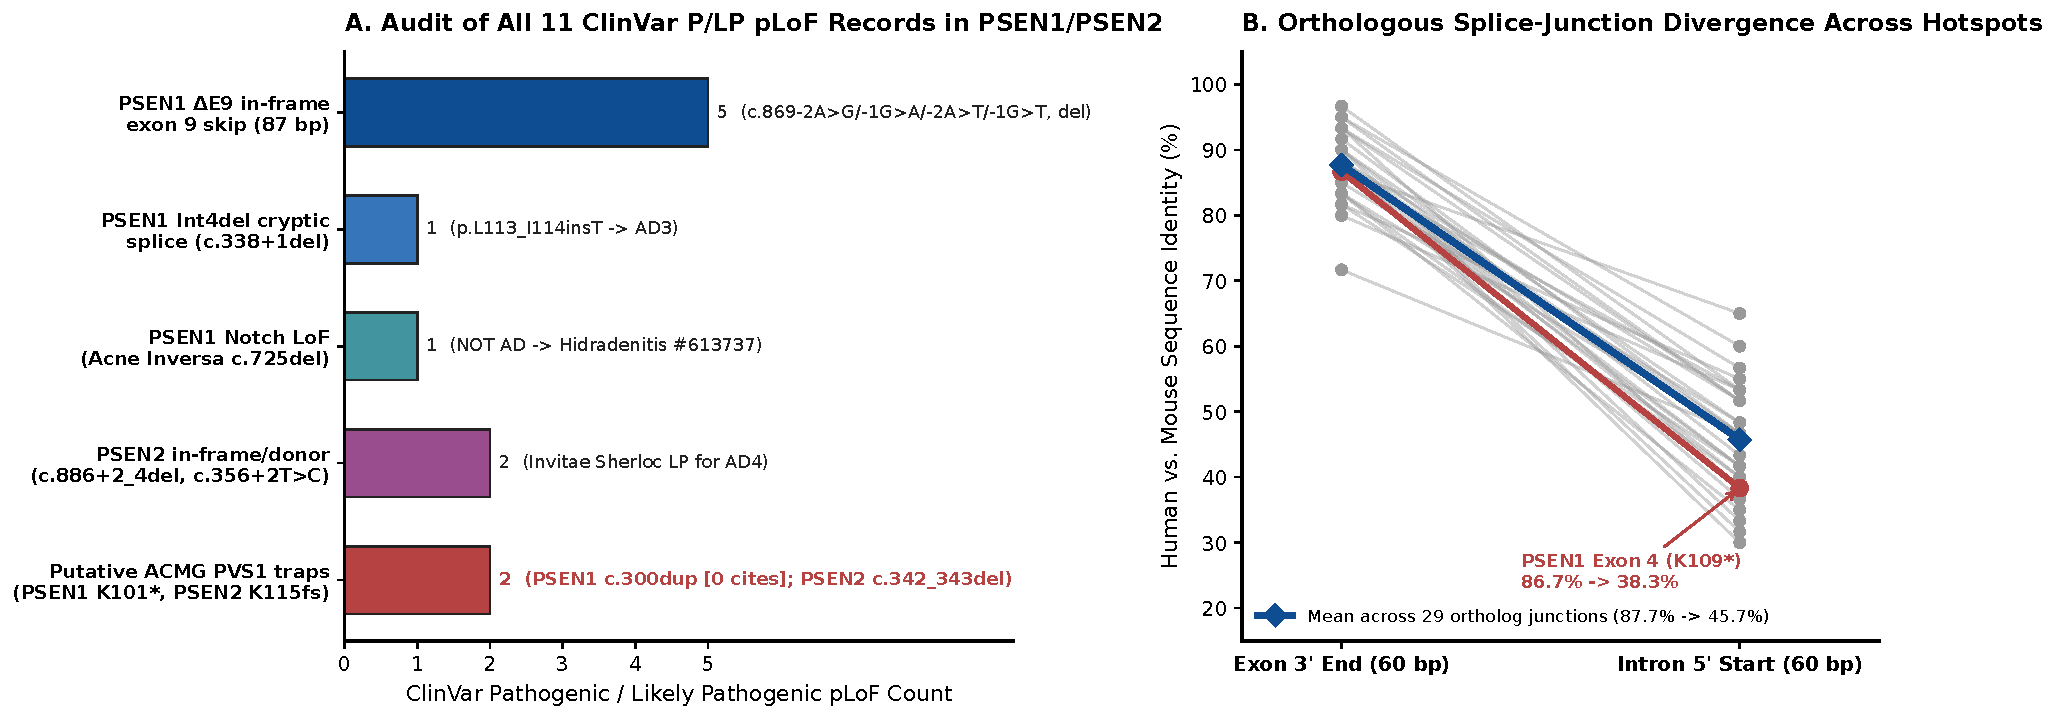
\includegraphics[width=0.96\textwidth,height=0.45\textheight,keepaspectratio]{figures/fig3_pvs1_audit_and_mouse_divergence.pdf}
  \caption{Evidence audit of ClinVar P/LP pLoF assertions and human--mouse junction conservation decay across conserved dementia gene exons. \textbf{(A)} Re-classification of all 11 ClinVar P/LP pLoF records in \textit{PSEN1} and \textit{PSEN2} separating verified pseudo-LoF splice events ($\Delta\text{E9}$, \texttt{c.338+1del}), non-ADAD allelic disorders (Acne Inversa), and uncorroborated or skippable-exon PVS1 liabilities. \textbf{(B)} Paired comparison across $n=29$ length-matched conserved coding exons comparing 60-bp exonic identity (mean 87.7\%, median 88.3\%) against adjacent 60-bp proximal intronic identity (mean 45.7\%, median 46.7\%) in human GRCh38 versus mouse GRCm39, illustrating \textit{PSEN1} Exon 4 divergence (86.7\% exonic to 38.3\% intronic).}
  \label{fig:fig3}
\end{figure}

Cross-species sequence alignment explained why rodent knock-in models routinely diverge from human splicing phenotypes (\textbf{Figure~\ref{fig:fig3}B}). Across $n=29$ length-matched conserved human--mouse exons ($|\Delta\text{len}| \leq 15$\,bp and exonic 60-bp identity $\geq 70\%$), terminal 60-bp coding identity remained tightly constrained (mean 87.7\%, median 88.3\%), whereas the immediately flanking 60-bp 5$'$ intronic sequence diverged catastrophically (mean 45.7\%, median 46.7%). At the \textit{PSEN1} Exon 4--Intron 4 boundary where \textit{Psen1}$^{\text{K109*/+}}$ mice fail to manifest EOAD amyloid pathology~\cite{sanjuanruiz2025,farinas2026}, human--mouse homology drops from 86.7\% across the 60-bp coding terminus to 38.3\% across the proximal intron (\texttt{c.325A>T} lies within a human intronic regulatory milieu poorly conserved in \textit{Mus musculus}).

\subsection{Cryo-EM Geometry, ESM-2 Fold Tolerance, and Allele-Selective Steric ASO Windows}
Mapping the cryptic-donor deletion \textit{PSEN1} p.K109\_L113del (\texttt{KDGQL}) onto the 2.6-\AA\ cryo-EM complex of human $\gamma$-secretase bound to APP-C83 (PDB ID \texttt{6IYC}) positioned the removed five residues squarely within hydrophilic loop 1 (HL1) at the ternary nicastrin--APP-C83 latch (\textbf{Figure~\ref{fig:fig4}A}). Flanking residues F105 and R108 anchor HL1 to nicastrin N243 (3.29\,\AA) and K654 (4.18\,\AA), while residues deleted or immediately adjacent make direct contacts with APP-C83—specifically D110--APP E6 (4.54\,\AA), G111--APP E6 (5.45\,\AA), Q112C--APP I16 (5.47\,\AA), and I114--APP V20 (3.77\,\AA)—whilst remaining 21.8--27.6\,\AA\ away from the catalytic dyad D257/D385~\cite{zhou2019}. Excising residues 109--113 short-circuits a 14.0-\AA\ C$\alpha$ span (R108--I114), predicting conformational distortion of the APP-C83 substrate clamp rather than active-site destruction, analogous to the distal Exon 9 $\Delta\text{E9}$ hinge region where S290 approaches APP L36 (7.97\,\AA).

\begin{figure}[!htb]
  \centering
  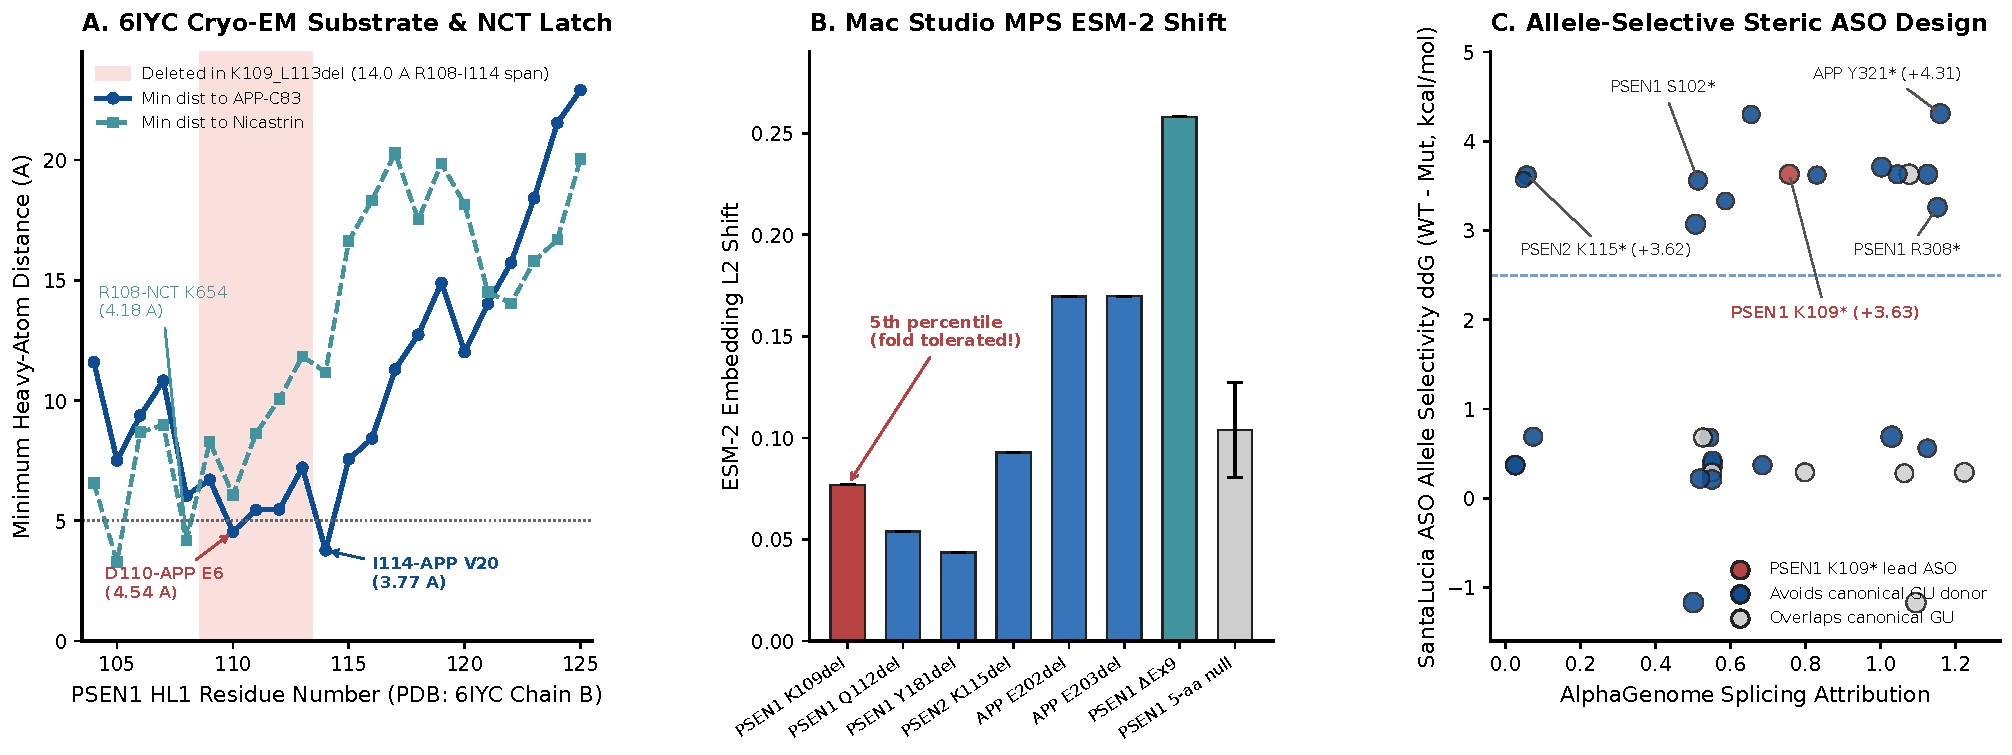
\includegraphics[width=0.96\textwidth,height=0.45\textheight,keepaspectratio]{figures/fig4_structure_6iyc_and_aso_thermodynamics.pdf}
  \caption{Structural geometry of \textit{PSEN1} HL1 in PDB 6IYC, ESM-2 fold-tolerance scoring on Apple Silicon MPS, and thermodynamic design of allele-selective steric ASOs. \textbf{(A)} Heavy-atom proximity of \textit{PSEN1} HL1 residues (Chain B, 104--125) to APP-C83 (Chain E, solid navy) and nicastrin (Chain A, dashed teal), highlighting the 14.0\,\AA\ R108--I114 span excised by p.K109\_L113del (pink shading). \textbf{(B)} Full-length ESM-2 (\texttt{esm2\_t12\_35M\_UR50D}) embedding L2 perturbation showing that \textit{PSEN1} p.K109\_L113del (0.0769, red) falls in the 5th percentile relative to 20 random 5-aa \textit{PSEN1} internal deletions ($0.1039 \pm 0.0236$), consistent with preserved global folding. \textbf{(C)} AlphaGenome splicing attribution plotted against SantaLucia nearest-neighbor allele selectivity ($\Delta\Delta G^\circ_{37} = \Delta G_{\text{WT}} - \Delta G_{\text{mut}}$) across 32 splice-hotspot targets, separating candidates avoiding canonical \texttt{+1/+2\,GU} donors (dark blue; lead \textit{PSEN1} p.K109* in red) from off-target GU-overlapping oligos (gray).}
  \label{fig:fig4}
\end{figure}

Orthogonal language-model evaluation with ESM-2 (\texttt{facebook/esm2\_t12\_35M\_UR50D}, PyTorch \texttt{mps}) corroborated structural fold preservation (\textbf{Figure~\ref{fig:fig4}B}). The cryptic deletion \textit{PSEN1} p.K109\_L113del yielded a global L2 embedding shift of 0.0769 ($\Delta\mathrm{PLL}=-0.00071$, flanking 10-aa $\mathrm{PLL}=-0.5018$), ranking at the 5th percentile of perturbation compared with 20 randomly positioned 5-amino-acid deletions across \textit{PSEN1} ($\mathrm{L2}=0.1039 \pm 0.0236$, $\text{mean flanking PLL}=-0.4557 \pm 0.1014$). Similarly mild global shifts occurred for \textit{PSEN2} p.K115\_L119del (\texttt{KNGQL}, $\mathrm{L2}=0.0929$), \textit{PSEN1} p.Q112\_L113del ($\mathrm{L2}=0.0540$), and p.Y181\_L182del ($\mathrm{L2}=0.0436$), in sharp contrast with the 29-aa Exon 9 deletion ($\mathrm{L2}=0.2580$) or the larger \textit{APP} Exon 5 acidic-domain deletions (20 aa p.E202\_S221del, $\mathrm{L2}=0.1697$).

Finally, thermodynamic tiling of 22-mer steric-blocking ASOs across all 32 prioritized stop-gain splicing hotspots (\textbf{Figure~\ref{fig:fig4}C}, \textbf{Table~\ref{tab:aso_panel}}) separated thermodynamically selective oligos that spare canonical \texttt{+1/+2\,GU} splice donors from non-selective windows that risk disrupting wild-type splicing. For \textit{PSEN1} c.325A$>$T (p.K109*), the lead candidate \texttt{5'-AGCUGCCCAUCCUACCGGGUAU-3'} spans the cryptic donor motif while terminating cleanly upstream of the canonical Intron 4 \texttt{+1/+2\,GU} dinucleotide (\textbf{Figure~\ref{fig:fig2}B}, green window), achieving a predicted mutant RNA--ASO $\Delta G^\circ_{37}=-45.92$\,kcal\,mol$^{-1}$ versus wild-type $-42.29$\,kcal\,mol$^{-1}$ ($\Delta\Delta G^\circ_{37}=+3.63$\,kcal\,mol$^{-1}$, $\Delta T_m=+15.6\,^\circ$C). Comparable selectivity windows avoiding canonical \texttt{GU} were recovered for \textit{PSEN1} c.305C$>$G (p.S102*, $+3.56$\,kcal\,mol$^{-1}$, $+16.0\,^\circ$C), \textit{PSEN1} p.R308* ($+3.26$\,kcal\,mol$^{-1}$, $+15.1\,^\circ$C), \textit{PSEN2} p.K115* ($+3.62$\,kcal\,mol$^{-1}$, $+15.7\,^\circ$C), and \textit{APP} p.Y321* ($+4.31$\,kcal\,mol$^{-1}$, $+16.9\,^\circ$C), whereas an initial hit at \textit{MAPT} p.G725* (\texttt{ACCUUCCACAGGGCUACAUGGU}) overlapped the canonical \texttt{+1/+2\,GU} donor ($\Delta\Delta G^\circ_{37}=+0.29$\,kcal\,mol$^{-1}$) and was penalized accordingly.

\begin{table}[!htb]
\centering
\caption{Selected 22-mer steric-blocking antisense oligonucleotide candidates avoiding canonical \texttt{+1/+2\,GU} donors from SantaLucia nearest-neighbor optimization ($\Delta\Delta G^\circ_{37} = \Delta G_{\text{WT}} - \Delta G_{\text{mut}}$).}
\label{tab:aso_panel}
\footnotesize
\setlength{\tabcolsep}{3pt}
\resizebox{\textwidth}{!}{%
\begin{tabular}{@{}llllcccc@{}}
\toprule
Gene & Variant (MANE) & Splicing $\mathrm{fi}$ & Lead ASO Sequence ($5'\rightarrow 3'$) & $\Delta G_{\text{mut}}$ & $\Delta G_{\text{WT}}$ & $\Delta\Delta G^\circ_{37}$ & $\Delta T_m$ ($^\circ$C) \\
\midrule
\textit{APP}   & c.963C$>$G (p.Y321*)  & 1.1596 & \texttt{UUGCCGCCACAUCCGCCCUAAA} & $-44.51$ & $-40.20$ & $+4.31$ & $+16.9$ \\
\textit{PSEN1} & c.922A$>$T (p.R308*)  & 1.1523 & \texttt{ACUCACCUUUGAGCUUCCGGGU} & $-42.93$ & $-39.67$ & $+3.26$ & $+15.1$ \\
\textit{MAPT}  & c.70A$>$T (p.K24*)    & 1.1259 & \texttt{UCUUACCUGUCCCCCAACCCGU} & $-45.42$ & $-41.79$ & $+3.63$ & $+15.6$ \\
\textit{PSEN1} & c.325A$>$T (p.K109*)  & 0.7569 & \texttt{AGCUGCCCAUCCUACCGGGUAU} & $-45.92$ & $-42.29$ & $+3.63$ & $+15.6$ \\
\textit{MAPT}  & c.1548C$>$G (p.Y516*) & 0.6550 & \texttt{GAAGUGACAGAAGAGACCUAUU} & $-37.03$ & $-32.73$ & $+4.30$ & $+16.9$ \\
\textit{PSEN1} & c.305C$>$G (p.S102*)  & 0.5132 & \texttt{GCUGACUCACUUAAUGGUAGCC} & $-40.96$ & $-37.40$ & $+3.56$ & $+16.0$ \\
\textit{PSEN2} & c.343A$>$T (p.K115*)  & 0.0570 & \texttt{GCUGUCCAUUCUACUCUGUGUA} & $-39.60$ & $-35.98$ & $+3.62$ & $+15.7$ \\
\bottomrule
\end{tabular}%
}
\end{table}

\section{Discussion}

Resolving whether autosomal-dominant dementia alleles operate by dosage deficiency or altered protein function bridges fundamental neurobiology and bedside precision medicine~\cite{menendez2004,menendezgonzalez2025,farinas2026}. Our pan-locus resource extends the paradigm established for \textit{PSEN1} by Farinas et al.~\cite{farinas2026} into a unified quantitative audit across \textit{PSEN1}, \textit{PSEN2}, \textit{APP}, \textit{MAPT}, and \textit{GRN}. Two decades after Men{\'e}ndez~\cite{menendez2004} emphasized that presenilin-1 mutations elicit striking neuropathological diversity—frequently defying linear structure--phenotype correlations—our structural and language-model data illustrate how non-missense alleles achieve conformational mimicry: splicing-mediated micro-deletions inside HL1 (\textit{PSEN1} p.K109\_L113del) or exon-9 hinges preserve global protein fold while selectively distorting the APP-C83 substrate clamp~\cite{zhou2019,yang2019}. Conversely, benign authentic null alleles stripped of cryptic splice rescue remain clinically silent for EOAD in general populations~\cite{farinas2026}, even when gene-level \texttt{pLI} nears unity owing to pleiotropic developmental selection or non-dementia phenotypes such as familial acne inversa~\cite{wang2010}.

These results highlight actionable safeguards for diagnostic variant interpretation and reporting. First, automated ACMG/AMP PVS1 pipelines~\cite{richards2015,aboutayoun2018} should remain active for \textit{GRN}, where 93.9\% of ClinVar P/LP burden reflects genuine haploinsufficiency, but should be disabled by default for canonical truncations in \textit{PSEN1}, \textit{PSEN2}, \textit{APP}, and \textit{MAPT}. In ClinVar, three Labcorp/Invitae submissions in \textit{PSEN2} currently hold Pathogenic or Likely Pathogenic tags despite $\mathrm{pLI}=0.0000$, 836 MANE coding pLoF alleles in gnomAD v4.1, and—in the case of \texttt{c.886+2\_886+4del}—a 99-bp in-frame skippable Exon 9. Second, in \textit{PSEN1}, nominal nonsense variants located anywhere near exon junctions or internal cryptic motifs—such as \texttt{c.300dup} (ClinVar ID 1027511) or predicted hotspots p.R308*, p.S102*, and p.Q29*—should never be dismissed as pure NMD nulls or assumed pathogenic without RNA splicing assays~\cite{baralle2005,dejonghe1999}; in our tridimensional etiological--molecular--clinical diagnostic model~\cite{menendezgonzalez2025}, orthogonal transcriptomics and A$\beta_{42}/A\beta_{38}$ readouts represent indispensable molecular proof. Third, our human--mouse alignment across 29 conserved exons (87.7\% exonic versus 45.7\% proximal intronic identity; \textit{PSEN1} Exon 4 dropping to 38.3\% intronic identity) suggests that mouse knock-in alleles lacking humanized introns~\cite{sanjuanruiz2025} cannot adjudicate human cryptic splicing safely—requiring patient-derived iPSC cortical neurons~\cite{arber2019} or humanized genomic constructs.

Therapeutically, the true-LoF versus pseudo-LoF distinction reshapes antisense strategy in opposite directions. Farinas et al.~\cite{farinas2026} observed that tolerance of heterozygous \textit{PSEN1} null alleles in humans de-risks cautious non-selective knockdown of \textit{PSEN1} or \textit{APP} (parallel to protective \textit{APP} cleavage reduction~\cite{jonsson2012}), provided Notch cleavage~\cite{yang2019} and follicular homeostasis~\cite{wang2010} are preserved. Yet when a nominal stop codon like \textit{PSEN1} p.K109* escapes NMD through cryptic splicing~\cite{farinas2026}, allele-selective steric-blocking splice-switching ASOs offer an orthogonal alternative: by masking the mutant cryptic donor (\texttt{5'-AGCUGCCCAUCCUACCGGGUAU-3'}, $\Delta\Delta G^\circ_{37}=+3.63$\,kcal\,mol$^{-1}$, sparing canonical \texttt{+1/+2\,GU}), an ASO is predicted in principle to sterically block aberrant splicing, reroute the mutant transcript back onto the native premature stop codon for benign NMD clearance, and leave wild-type \textit{PSEN1} expression intact.

Several methodological boundaries must be underscored. First, AlphaGenome AVI attributions~\cite{avsec2026,alphagenome_atlas2026}, ESM-2 likelihoods~\cite{lin2023}, and SantaLucia unmodified duplex $\Delta G^\circ_{37}$ estimates~\cite{santalucia1998} are purely \textit{in silico} models; chemical modifications used clinically (2$'$-O-methoxyethyl, phosphorothioate, or locked nucleic acids) alter steric affinity, RNase H1 recruitment risk, and specificity relative to unmodified RNA thermodynamics. Second, PDB 6IYC incorporates engineered disulfide crosslinks (\textit{PSEN1} Q112C and APP V8C) and lacks electron density for parts of the Exon 9 hinge (residues 308--319), limiting direct modeling of p.R308* skip isoforms~\cite{zhou2019}. Third, long-read cDNA sequencing (RT-PCR or nanopore Iso-Seq) in carrier lymphoblasts or iPSC neurons paired with mass-spectrometric A$\beta_{37/38/40/42/43}$ processivity profiling remains mandatory before any diagnostic reclassification or therapeutic translation~\cite{arber2019,farinas2026}.

\section{Conclusions}

Across 1,092 MANE Select stop-gain variants in five major dementia genes, authentic NMD-sensitive loss-of-function mutations in \textit{PSEN1}, \textit{PSEN2}, \textit{APP}, and \textit{MAPT} remain mechanistically distinct from \textit{GRN} haploinsufficiency, while a reproducible subset of nominal truncations activates cryptic splice donors or modular exon skipping to mimic missense-like gain-of-function. Correcting ACMG PVS1 curation rules, prioritizing human splicing models over murine intronic orthologs, and exploiting cryptic-donor steric ASO windows turn a diagnostic pitfall into an actionable precision-medicine framework.

\section*{Data and Code Availability}
All genomic annotations, sequence architectures, summary statistics, and pipeline outputs were derived from publicly accessible resources: Ensembl GRCh38 and GRCm39 REST APIs, the AlphaGenome Atlas variant portal, gnomAD v4.1, NCBI ClinVar, and the RCSB Protein Data Bank (\texttt{6IYC}). All self-contained Python pipeline scripts, GeneForge Language catalog specifications (\texttt{five\_gene\_pseudolof\_aso\_catalog.gfl}), derived JSON/TSV tables, and figure generation scripts required to reproduce every quantitative value and figure reported in this manuscript are packaged in the accompanying Supplementary Archive (\texttt{Supplementary\_Data\_and\_Code.zip}).

\section*{Artificial Intelligence and Bioinformatics Disclosure}
Autonomous bioinformatic orchestration frameworks (declarative genomic catalog specification and AlphaGenome Atlas API integration) were used alongside generative AI assistance for Python pipeline automation, manuscript preparation, and LaTeX formatting. All computational outputs, statistical calculations, database records, citations, and structural interpretations were verified empirically against primary public databases, and the author holds full epistemic, scientific, and intellectual responsibility for all content.

\section*{Competing Interests}
The author declares no competing financial or non-financial interests.

\bibliographystyle{unsrt}
\bibliography{references}

\end{document}
